\documentclass{standalone}
\usepackage{tikz}
\usepackage{xcolor}
\usetikzlibrary{patterns, positioning}
\usetikzlibrary{shapes.misc}
\usepackage[outline]{contour}
\contourlength{1.5pt} 


\begin{document}
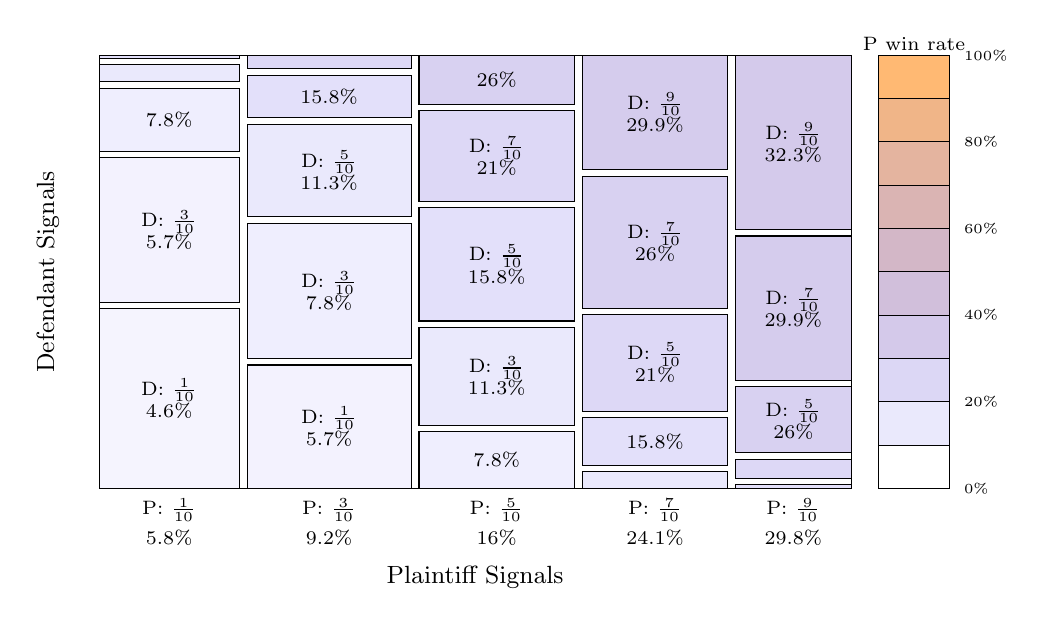
\begin{tikzpicture}
\newcommand{\DFractionOffset}{0.4}
\newcommand{\AxisLabelYAdjust}{-0.235}
\draw[draw=black] (0.6,2) rectangle (10.15,7.5);
\draw[fill=blue!95!orange!5!white!86!white, draw=black] (0.6,2) rectangle (2.3787,4.2843);
\draw (1.489333849105874, 3.1421451019850517) node[font=\scriptsize, text=black, align=center] {D: $\frac{1}{10}$\\ 4.6\%};
\draw[fill=blue!94!orange!6!white!86!white, draw=black] (0.6,4.3643) rectangle (2.3787,6.2004);
\draw (1.489333849105874, 5.282339448338528) node[font=\scriptsize, text=black, align=center] {D: $\frac{3}{10}$\\ 5.7\%};
\draw[fill=blue!92!orange!8!white!85!white, draw=black] (0.6,6.2804) rectangle (2.3787,7.0826);
\draw (1.489333849105874, 6.681495358257184) node[font=\scriptsize, text=black, align=center] {7.8\%};
\draw[fill=blue!89!orange!11!white!84!white, draw=black] (0.6,7.1626) rectangle (2.3787,7.3803);
\draw[fill=blue!84!orange!16!white!83!white, draw=black] (0.6,7.4603) rectangle (2.3787,7.5);
\draw (1.489333849105874, 1.6) node[anchor=north, font=\scriptsize, text=black] {5.8\%};
\draw (1.489333849105874, {1.6 + \DFractionOffset}) node[anchor=north, font=\scriptsize, text=black] {P: $\frac{1}{10}$};
\draw[fill=blue!94!orange!6!white!86!white, draw=black] (2.4787,2) rectangle (4.5626,3.5671);
\draw (3.5206333002273125, 2.783569310333831) node[font=\scriptsize, text=black, align=center] {D: $\frac{1}{10}$\\ 5.7\%};
\draw[fill=blue!92!orange!8!white!85!white, draw=black] (2.4787,3.6471) rectangle (4.5626,5.3687);
\draw (3.5206333002273125, 4.507914100632646) node[font=\scriptsize, text=black, align=center] {D: $\frac{3}{10}$\\ 7.8\%};
\draw[fill=blue!89!orange!11!white!84!white, draw=black] (2.4787,5.4487) rectangle (4.5626,6.6257);
\draw (3.5206333002273125, 6.037211891673656) node[font=\scriptsize, text=black, align=center] {D: $\frac{5}{10}$\\ 11.3\%};
\draw[fill=blue!84!orange!16!white!83!white, draw=black] (2.4787,6.7057) rectangle (4.5626,7.2481);
\draw (3.5206333002273125, 6.976939136137375) node[font=\scriptsize, text=black, align=center] {15.8\%};
\draw[fill=blue!79!orange!21!white!81!white, draw=black] (2.4787,7.3281) rectangle (4.5626,7.5);
\draw (3.5206333002273125, 1.6) node[anchor=north, font=\scriptsize, text=black] {9.2\%};
\draw (3.5206333002273125, {1.6 + \DFractionOffset}) node[anchor=north, font=\scriptsize, text=black] {P: $\frac{3}{10}$};
\draw[fill=blue!92!orange!8!white!85!white, draw=black] (4.6626,2) rectangle (6.6363,2.7229);
\draw (5.649445500266767, 2.361472325577367) node[font=\scriptsize, text=black, align=center] {7.8\%};
\draw[fill=blue!89!orange!11!white!84!white, draw=black] (4.6626,2.8029) rectangle (6.6363,4.0457);
\draw (5.649445500266767, 3.4243380930411065) node[font=\scriptsize, text=black, align=center] {D: $\frac{3}{10}$\\ 11.3\%};
\draw[fill=blue!84!orange!16!white!83!white, draw=black] (4.6626,4.1257) rectangle (6.6363,5.5661);
\draw (5.649445500266767, 4.845891093202244) node[font=\scriptsize, text=black, align=center] {D: $\frac{5}{10}$\\ 15.8\%};
\draw[fill=blue!79!orange!21!white!81!white, draw=black] (4.6626,5.6461) rectangle (6.6363,6.7955);
\draw (5.649445500266767, 6.220781847262938) node[font=\scriptsize, text=black, align=center] {D: $\frac{7}{10}$\\ 21\%};
\draw[fill=blue!74!orange!26!white!79!white, draw=black] (4.6626,6.8755) rectangle (6.6363,7.5);
\draw (5.649445500266767, 7.187756521524433) node[font=\scriptsize, text=black, align=center] {26\%};
\draw (5.649445500266767, 1.6) node[anchor=north, font=\scriptsize, text=black] {16\%};
\draw (5.649445500266767, {1.6 + \DFractionOffset}) node[anchor=north, font=\scriptsize, text=black] {P: $\frac{5}{10}$};
\draw[fill=blue!89!orange!11!white!84!white, draw=black] (6.7363,2) rectangle (8.584,2.2096);
\draw[fill=blue!84!orange!16!white!83!white, draw=black] (6.7363,2.2896) rectangle (8.584,2.9013);
\draw (7.660170624249327, 2.5954216304398536) node[font=\scriptsize, text=black, align=center] {15.8\%};
\draw[fill=blue!79!orange!21!white!81!white, draw=black] (6.7363,2.9813) rectangle (8.584,4.2091);
\draw (7.660170624249327, 3.5951937792130773) node[font=\scriptsize, text=black, align=center] {D: $\frac{5}{10}$\\ 21\%};
\draw[fill=blue!74!orange!26!white!79!white, draw=black] (6.7363,4.2891) rectangle (8.584,5.9663);
\draw (7.660170624249327, 5.127692018343058) node[font=\scriptsize, text=black, align=center] {D: $\frac{7}{10}$\\ 26\%};
\draw[fill=blue!70!orange!30!white!78!white, draw=black] (6.7363,6.0463) rectangle (8.584,7.5);
\draw (7.660170624249327, 6.7731437766899845) node[font=\scriptsize, text=black, align=center] {D: $\frac{9}{10}$\\ 29.9\%};
\draw (7.660170624249327, 1.6) node[anchor=north, font=\scriptsize, text=black] {24.1\%};
\draw (7.660170624249327, {1.6 + \DFractionOffset}) node[anchor=north, font=\scriptsize, text=black] {P: $\frac{7}{10}$};
\draw[fill=blue!84!orange!16!white!83!white, draw=black] (8.684,2) rectangle (10.15,2.0482);
\draw[fill=blue!79!orange!21!white!81!white, draw=black] (8.684,2.1282) rectangle (10.15,2.3725);
\draw[fill=blue!74!orange!26!white!79!white, draw=black] (8.684,2.4525) rectangle (10.15,3.2933);
\draw (9.417024575103998, 2.872870218054695) node[font=\scriptsize, text=black, align=center] {D: $\frac{5}{10}$\\ 26\%};
\draw[fill=blue!70!orange!30!white!78!white, draw=black] (8.684,3.3733) rectangle (10.15,5.2056);
\draw (9.417024575103998, 4.2894269938883465) node[font=\scriptsize, text=black, align=center] {D: $\frac{7}{10}$\\ 29.9\%};
\draw[fill=blue!68!orange!32!white!77!white, draw=black] (8.684,5.2856) rectangle (10.15,7.5);
\draw (9.417024575103998, 6.392796287558075) node[font=\scriptsize, text=black, align=center] {D: $\frac{9}{10}$\\ 32.3\%};
\draw (9.417024575103998, 1.6) node[anchor=north, font=\scriptsize, text=black] {29.8\%};
\draw (9.417024575103998, {1.6 + \DFractionOffset}) node[anchor=north, font=\scriptsize, text=black] {P: $\frac{9}{10}$};
\node[font=\small, text=black] at (5.375, {1.1 + \AxisLabelYAdjust}) {Plaintiff Signals};
\node[font=\small, text=black, rotate=90] at (-0.050000000000000044, 4.75) {Defendant Signals};
\draw[draw=black] (10.5,2) rectangle (11.4,7.5);
\draw (10.95, 7.65) node[font=\scriptsize, text=black] {P win rate};
\draw[fill=blue!100!orange!0!white!88!white, draw=black] (10.5,2) rectangle (11.4,2.55);
\draw[fill=blue!89!orange!11!white!84!white, draw=black] (10.5,2.55) rectangle (11.4,3.1);
\draw[fill=blue!78!orange!22!white!81!white, draw=black] (10.5,3.1) rectangle (11.4,3.65);
\draw[fill=blue!67!orange!33!white!77!white, draw=black] (10.5,3.65) rectangle (11.4,4.2);
\draw[fill=blue!56!orange!44!white!73!white, draw=black] (10.5,4.2) rectangle (11.4,4.75);
\draw[fill=blue!44!orange!56!white!70!white, draw=black] (10.5,4.75) rectangle (11.4,5.3);
\draw[fill=blue!33!orange!67!white!66!white, draw=black] (10.5,5.3) rectangle (11.4,5.85);
\draw[fill=blue!22!orange!78!white!62!white, draw=black] (10.5,5.85) rectangle (11.4,6.4);
\draw[fill=blue!11!orange!89!white!59!white, draw=black] (10.5,6.4) rectangle (11.4,6.95);
\draw[fill=blue!0!orange!100!white!55!white, draw=black] (10.5,6.95) rectangle (11.4,7.5);
\draw (11.46, 2) node[anchor=west, font=\tiny, text=black] {0\%};
\draw (11.46, 3.1) node[anchor=west, font=\tiny, text=black] {20\%};
\draw (11.46, 4.2) node[anchor=west, font=\tiny, text=black] {40\%};
\draw (11.46, 5.3) node[anchor=west, font=\tiny, text=black] {60\%};
\draw (11.46, 6.4) node[anchor=west, font=\tiny, text=black] {80\%};
\draw (11.46, 7.5) node[anchor=west, font=\tiny, text=black] {100\%};


\end{tikzpicture}
\end{document}